% \section{IMU误差模型}
\section{近期IMU应用中的问题及解决}

%%%%%%%%%%%%%%%%%%%%%%%%%%%%

\begin{frame}[fragile]
  \frametitle{近期IMU应用中的问题及解决(一) \hfill 
\includegraphics[height=0.5cm]{00_logo.png}}
  \begin{columns}
    \column{0.1\textwidth}
    
    \column{0.8\textwidth}
    \begin{itemize}
      \item 问题一:同样是右手坐标系,不同的是$z$轴上的数值取反(原来重力大小为-9.8,需要改成9.8),有两种方式.

      \item 方式一:
      
      \begin{lstlisting}[frame=shadowbox]  
        // pentu_ig1.urdf
        <joint name="imu_link_joint" type="fixed">
          <parent link="base_footprint" />
          <child link="imu" />
          <origin xyz="0 0 0" rpy="3.14 0 0"/>
        </joint>
      \end{lstlisting}

      \begin{lstlisting}[frame=shadowbox]  
        // SensorBridge::HandleImuMessage()
        imu_data->angular_velocity = Eigen::Vector3d{imu_data->angular_velocity[0], 
            -imu_data->angular_velocity[1], -imu_data->angular_velocity[2]};
        imu_data->linear_acceleration = Eigen::Vector3d{imu_data->linear_acceleration[0],
            -imu_data->linear_acceleration[1], imu_data->linear_acceleration[2]};    
        ......    
        trajectory_builder_->AddSensorData( sensor_id,
            carto::sensor::ImuData{imu_data->time, imu_data->linear_acceleration,
                               imu_data->angular_velocity});
      \end{lstlisting}

    \end{itemize}
    
    % \column{0.3\textwidth}
    % \begin{figure}[h]
    %   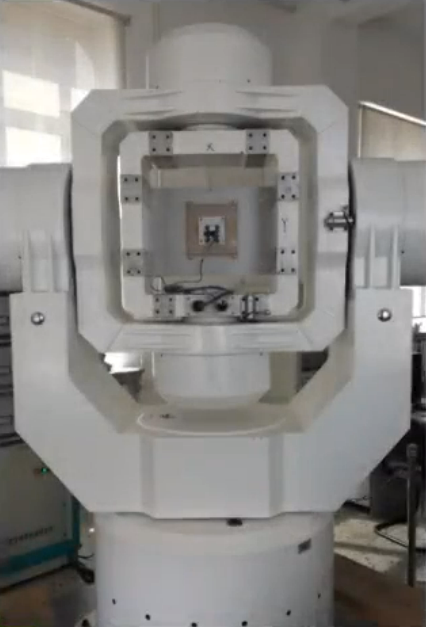
\includegraphics[trim=1.5 0 0 0, height=3.5cm,clip]{12_1.png}
    %   % \caption{四个区域搜索空间}
    % \end{figure}

    \column{0.1\textwidth}
  
  \end{columns}
  \end{frame}   

  %%%%%%%%%%%%%%%%%%%%%%%%%%%%

\begin{frame}[fragile]
  \frametitle{近期IMU应用中的问题及解决(一) \hfill 
\includegraphics[height=0.5cm]{00_logo.png}}
  \begin{columns}
    \column{0.1\textwidth}
    
    \column{0.8\textwidth}
    \begin{itemize}
      \item 方式二:
      
      \begin{lstlisting}[frame=shadowbox]  
        // pentu_ig1.urdf
        <joint name="imu_link_joint" type="fixed">
          <parent link="base_footprint" />
          <child link="imu" />
          <origin xyz="0 0 0" rpy="0 0 0"/>
        </joint>
      \end{lstlisting}

      \begin{lstlisting}[frame=shadowbox]  
        // SensorBridge::HandleImuMessage()
        imu_data->linear_acceleration[2] = -imu_data->linear_acceleration[2];    
        ......    
        trajectory_builder_->AddSensorData( sensor_id,
            carto::sensor::ImuData{imu_data->time, imu_data->linear_acceleration,
                               imu_data->angular_velocity});
      \end{lstlisting}

    \end{itemize}
    
    % \column{0.3\textwidth}
    % \begin{figure}[h]
    %   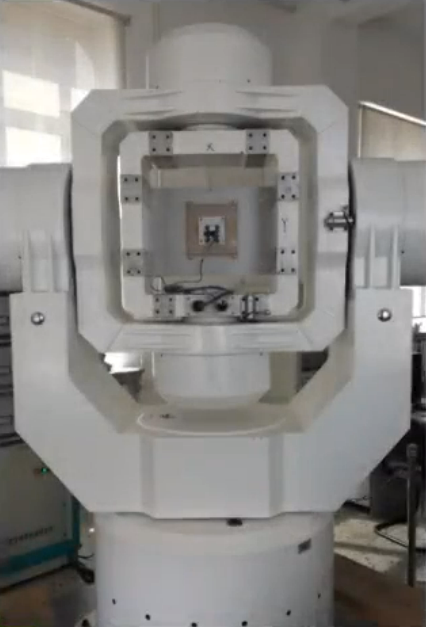
\includegraphics[trim=1.5 0 0 0, height=3.5cm,clip]{12_1.png}
    %   % \caption{四个区域搜索空间}
    % \end{figure}

    \column{0.1\textwidth}
  
  \end{columns}
  \end{frame}   


  %%%%%%%%%%%%%%%%%%%%%%%%%%%%

\begin{frame}[fragile]
  \frametitle{近期IMU应用中的问题及解决(二) \hfill 
\includegraphics[height=0.5cm]{00_logo.png}}
  \begin{columns}
    \column{0.1\textwidth}
    
    \column{0.8\textwidth}
    \begin{itemize}
      \item 问题二:IMU安装不是不水平的,base\_footprint到imu的静态TF的标定困难.解决方法是开发一个自动标定IMU的代码.

      
      \begin{lstlisting}[frame=shadowbox]  
        // pentu_ig1.urdf
        <joint name="imu_link_joint" type="fixed">
          <parent link="base_footprint" />
          <child link="imu" />
          <origin xyz="0 0 0" rpy="-0.00478014 -0.000399168 0"/>
        </joint>

      \end{lstlisting}

    \end{itemize}
    
    % \column{0.3\textwidth}
    % \begin{figure}[h]
    %   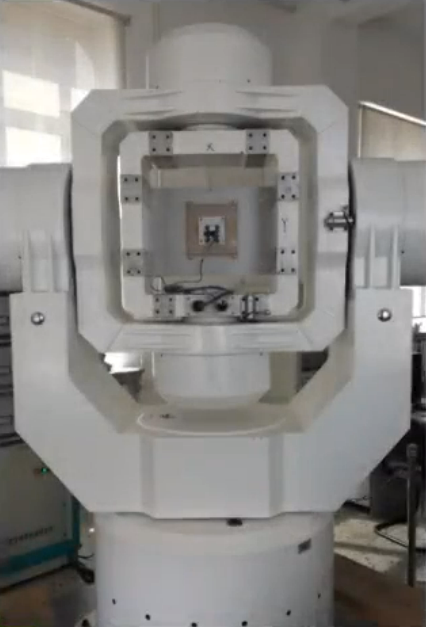
\includegraphics[trim=1.5 0 0 0, height=3.5cm,clip]{12_1.png}
    %   % \caption{四个区域搜索空间}
    % \end{figure}

    \column{0.1\textwidth}
  
  \end{columns}
  \end{frame}   

%%%%%%%%%%%%%%%%%%%%%%%%%%%%

\begin{frame}[fragile]
  \frametitle{近期IMU应用中的问题及解决(二) \hfill 
\includegraphics[height=0.5cm]{00_logo.png}}
  \begin{columns}
    \column{0.1\textwidth}
    
    \column{0.8\textwidth}
      \begin{lstlisting}[frame=shadowbox]  
        void ImuCallback(const sensor_msgs::ImuConstPtr& msg)
        {
          static int nums = 0;
          static Eigen::Vector3d calibr_sum;
          if(++nums > 500)
            return;
          if(nums <= 500)
          {
            std::unique_ptr<cartographer::sensor::ImuData> imu_data = ToImuData(msg);
            const Eigen::Quaterniond rotation = Eigen::Quaterniond::FromTwoVectors(
              imu_data->linear_acceleration, Eigen::Vector3d{0, 0, -9.8});  
            Eigen::Vector3d calibr = cartographer::transform::RotationQuaternionToAngleAxisVector(rotation);
            calibr_sum += calibr;
          }
          if(nums == 500)
              std::cout << "[rpy:]" << calibr_sum / 500 << std::endl;
        }
      \end{lstlisting}

    
    % \column{0.3\textwidth}
    % \begin{figure}[h]
    %   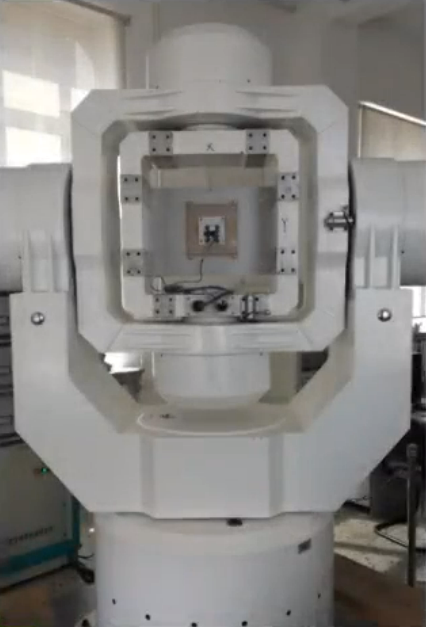
\includegraphics[trim=1.5 0 0 0, height=3.5cm,clip]{12_1.png}
    %   % \caption{四个区域搜索空间}
    % \end{figure}

    \column{0.1\textwidth}
  
  \end{columns}
  \end{frame}   

